\documentclass{math}

\usepackage{tikz}

\geometry{letterpaper, margin=0.5in}

\title{Multivariable and Vector Calculus: Homework 12}
\author{Alvin Lin}
\date{August 2016 - December 2016}

\begin{document}

\maketitle

\section*{Section 16.9}

\subsubsection*{Exercise 7}
Use the Divergence Theorem to calculate the surface integral
\( \iint_{S}F\cdot\diff{S} \); that is, calculate the flux of \( F \) across
\( S \).
\[ F(x,y,z) = 3xy^2\i+x\e^z\j+z^3\k \]
\( S \) is the surface of the solid bounded by the cylinder \( y^2+z^2 = 1 \)
and the planes \( x = -1 \) and \( x = 2 \).
\begin{align*}
  \iint_{S}F\diff{S} &= \iiint_{E}\text{div}~F\diff{V} \\
  \text{div}~F &= 3y^2+0+3z^2 \\
  3\iiint_{E}y^2+z^2\diff{V} &=
    3\int_{-1}^{2}\int_{0}^{2\pi}\int_{0}^{1}(r\cos\theta)^2+(r\sin\theta)^2r
    \diff{r}\diff{\theta}\diff{z} \\
  &= 3\int_{-1}^{2}\int_{0}^{2\pi}\int_{0}^{1}r^3(\cos^2\theta+\sin^2\theta)
    \diff{r}\diff{\theta}\diff{z} \\
  &= 3\int_{-1}^{2}\int_{0}^{2\pi}\bigg[\frac{r^4}{4}\bigg]_{0}^{1}
    \diff{\theta}\diff{z} \\
  &= \frac{3}{4}\int_{-1}^{2}\int_{0}^{2\pi}\diff{\theta}\diff{z} \\
  &= \frac{3}{4}\int_{-1}^{2}\bigg[\theta\bigg]_{0}^{2\pi}\diff{z} \\
  &= \frac{6\pi}{4}\int_{-1}^{2}\diff{z} \\
  &= \frac{3\pi}{2}\bigg[z\bigg]_{-1}^{2} \\
  &= \frac{9\pi}{2}
\end{align*}

\subsubsection*{Exercise 11}
Use the Divergence Theorem to calculate the surface integral
\( \iint_{S}F\cdot\diff{S} \); that is, calculate the flux of \( F \) across
\( S \).
\[ F(x,y,z) = (2x^3+y^3)\i+(y^3+z^3)\j+3y^2z\k \]
\( S \) is the surface of the solid bounded by the paraboloid
\( z = 1-x^2-y^2 \) and the xy-plane.
\begin{align*}
  \iint_{S}F\diff{S} &= \iiint_{E}\text{div}~F\diff{V} \\
  \text{div}~F &= 6x^2+3y^2+3y^2 \\
  &= 6(x^2+y^2) \\
  \iiint_{E}6(x^2+y^2)\diff{V} &= 6\int_{0}^{2\pi}\int_{0}^{1}\int_{0}^{1-r^2}
    r^2r\diff{z}\diff{r}\diff{\theta} \\
  &= 6\int_{0}^{2\pi}\int_{0}^{1}r^3\bigg[z\bigg]_{0}^{1-r^2}
    \diff{r}\diff{\theta} \\
  &= 6\int_{0}^{2\pi}\int_{0}^{1}r^3(1-r^2)\diff{r}\diff{\theta} \\
  &= 6\int_{0}^{2\pi}\bigg[\frac{r^4}{4}-\frac{r^6}{6}\bigg]_{0}^{1}
    \diff{\theta} \\
  &= 6\int_{0}^{2\pi}\frac{1}{4}-\frac{1}{6}\diff{\theta} \\
  &= \frac{6}{12}\int_{0}^{2\pi}\diff{\theta} \\
  &= \frac{2\pi}{2} = \pi \\
\end{align*}

\subsubsection*{Exercise 17}
Use the Divergence Theorem to evaluate \( \iint_{S}F\cdot\diff{S} \), where
\( F(x,y,z) = z^2x\i+(\frac{1}{3}y^3+\tan(z))\j+(x^2z+y^2)\k \) and \( S \) is
the top half of the sphere \( x^2+y^2+z^2 = 1 \). Note that \( S \) is not a
closed surface. First compute integrals over \( S_1 \) and \( S_2 \), where
\( S_1 \) is the disk \( x^2+y^2\le1 \), oriented downward, and
\( S_2 = S\cup S_1 \).
\begin{align*}
  \iint_{S}F\diff{S} &= \iiint_{E}\text{div}~F\diff{V} \\
  \text{div}~F &= z^2+y^2+x^2 \\
  \iint_{S_1}F\diff{S} &=
    \iint_{D}F\cdot(-\k)\sqrt{(\pdiff{z}{x})^2+(\pdiff{z}{y})^2+1}\diff{A} \\
  &= -\iint_{D}(x^2z+y^2)\sqrt{1}\diff{A} \\
  &= -\int_{0}^{2\pi}\int_{0}^{1}(r\cos\theta)^2(0)+(r\sin\theta)^2r
    \diff{r}\diff{\theta} \\
  &= -\int_{0}^{2\pi}\sin^2\theta\int_{0}^{1}r^3\diff{r}\diff{\theta} \\
  &= -\int_{0}^{2\pi}\sin^2\theta\bigg[\frac{r^4}{4}\bigg]_{0}^{1}
    \diff{\theta}
\end{align*}
\begin{align*}
  &= -\frac{1}{4}\int_{0}^{2\pi}\frac{1-\cos(2\theta)}{2}\diff{\theta} \\
  &= -\frac{1}{8}\bigg[\theta-\frac{\sin2\theta}{2}\bigg]_{0}^{2\pi} \\
  &= -\frac{2\pi}{8} = -\frac{\pi}{4}
\end{align*}

\subsubsection*{Exercise 25}
Prove each identity, assuming that \( S \) and \( E \) satisfy the conditions of
the Divergence Theorem and the scalar functions and components of the vector
fields have continouous second-order partial derivatives.
\[ \iint_{S}a\cdot n\diff{S} = 0 \]
where \( \vec{a} \) is a constant vector.
\begin{align*}
  \text{div}~\vec{a} &= 0 \\
  \iint_{S}\vec{a}\cdot n\diff{S} &= \iiint_{E}0\diff{V} = 0
\end{align*}

\subsubsection*{Exercise 27}
Prove each identity, assuming that \( S \) and \( E \) satisfy the conditions of
the Divergence Theorem and the scalar functions and components of the vector
fields have continouous second-order partial derivatives.
\[ \iint_{S}\text{curl}~F\cdot\diff{S} = 0 \]
\begin{align*}
  \iint_{S}\text{curl}~F\cdot\diff{S} &=
    \iiint_{E}\text{div}(\text{curl}~F)\diff{V} \\
  &= \iint_{E}\triangledown\cdot(\triangledown\times F)\diff{V} \\
  &= \iiint_{E}0\diff{V} \\
  &= 0
\end{align*}

\section*{Section 16.8}

\subsubsection*{Exercise 5}
Use Stokes' Theorem to evaluate \( \iint_{S}\text{curl}~F\cdot\diff{S} \).
\[ F(x,y,z) = xyz\i+xy\j+x^2yz\k \]
\( S \) consists of the top and the four sides (but not the bottom) of the cube
with vertices \( (\pm1,\pm1,\pm1) \), oriented outward.
\begin{align*}
  \iint_{S}\text{curl}~\diff{S} &=
    \iint_{H}\text{curl}~F\k\diff{S} \\
  &= \iint_{H}\pdiff{Q}{x}-\pdiff{P}{y}\diff{S} \\
  &= \iint_{H}y-zx\diff{S} \\
  &= \iint_{S}y+x\diff{S} \\
  &= \int_{-1}^{1}\int_{-1}^{1}y+x\diff{x}\diff{y} \\
  &= \int_{-1}^{1}\bigg[yx+\frac{x^2}{2}\bigg]_{-1}^{1}\diff{y} \\
  &= \int_{-1}^{1}2y\diff{y} \\
  &= 0
\end{align*}

\subsubsection*{Exercise 9}
Use Stokes' Theorem to evaluate \( \int_{C}F\cdot\diff{r} \). In each case
\( C \) is oriented counterclockwise as viewed from above.
\[ F(x,y,z) = xy\i+yz\j+zx\k \]
\( C \) is the boundary of the part of the paraboloid \( 1-x^2-y^2 \) in the
first octant.
\begin{align*}
  \int_{C}F\cdot\diff{r} &= \iint_{S}\text{curl}~F\diff{S} \\
  &= \iint_{D}-P(\pdiff{g}{x})-Q(\pdiff{g}{y})+R\diff{A} \\
  &= \iint_{D}y(-2x)-(-z)(-2y)-x\diff{A} \\
  &= \iint_{D}-2xy-2yz-x\diff{A} \\
  &= \iint_{D}-2xy-2y(1-x^2-y^2)-x\diff{A} \\
  &= \iint_{D}-2xy-2y+2yx^2+2y^3-x\diff{A} \\
  &= \iint_{D}-2y(x+1-x^2-y^2)-x\diff{A} \\
\end{align*}
\begin{align*}
  &= \int_{0}^{\frac{\pi}{2}}\int_{0}^{1}
    (-2r\cos\theta(r\sin\theta+1-r^2)-r\cos\theta)r\diff{r}\diff{\theta} \\
  &= \int_{0}^{\frac{\pi}{2}}\int_{0}^{1}
    -2r^3\cos\theta\sin\theta-2r\cos\theta+2r^4\cos\theta-r^2\cos\theta
    \diff{r}\diff{\theta} \\
  &= \int_{0}^{\frac{\pi}{2}}\int_{0}^{1}
    -r^3\sin2\theta-2r\cos\theta+2r^4\cos\theta-r^2\cos\theta
    \diff{r}\diff{\theta} \\
  &= \int_{0}^{\frac{\pi}{2}}
    \bigg[\frac{-r^4\sin2\theta}{4}-\frac{2r^3\sin\theta}{3}+
    \frac{2r^5\sin\theta}{5}-\frac{r^3\cos\theta}{3}\bigg]_{0}^{1}
    \diff{\theta} \\
  &= \int_{0}^{\frac{\pi}{2}}
    -\frac{\sin2\theta}{4}-\frac{2\sin\theta}{3}+\frac{2\sin\theta}{5}-
    \frac{\cos\theta}{3}\diff{\theta} \\
  &= \bigg[\frac{1}{2}\frac{\cos2\theta}{4}+\frac{2\cos\theta}{3}-
    \frac{2\cos\theta}{5}-\frac{\sin\theta}{3}\bigg]_{0}^{\frac{\pi}{2}} \\
  &= (-\frac{1}{8}+0-0-\frac{1}{3})-(\frac{1}{8}+\frac{2}{3}-\frac{2}{5}-0) \\
  &= -\frac{17}{20}
\end{align*}

\subsubsection*{Exercise 15}
Verify that Stokes' Theorem is true for the given vector field \( F \) and
surface \( S \).
\[ F(x,y,z) = y\i+z\j+x\k \]
\( S \) is the hemisphere \( x^2+y^2+z^2 = 1 \), \( y\ge0 \), oriented in the
direction of the positive y-axis.
\[ ? \]

\subsubsection*{Exercise 17}
A particle moves along line segments from the origin to the points (1,0,0),
(1,2,1), (0,2,1), and back to the origin under the influence of the force field
\[ F(x,y,z) = z^2\i+2xy\j+4y^2\k \]
Find the work done.
\begin{align*}
  \int_{C}F\cdot\diff{r} &= \iint_{S}\text{curl}~F\diff{S} \\
  &= \iint_{D}-P(\pdiff{g}{x})-Q(\pdiff{g}{y})+R\diff{A} \\
  &= \iint_{D}-8y(\pdiff{g}{x})-2z(\pdiff{g}{y})+2y\diff{A} \\
  &= \iint_{D}0-z+2y\diff{A} \\
  &= \iint_{D}0-\frac{y}{2}+2y\diff{A} \\
  &= \iint_{D}\frac{3y}{2}\diff{A} \\
  &= \frac{3}{2}\int_{0}^{1}\int_{0}^{2}y\diff{y}\diff{x} \\
  &= \frac{3}{2}\int_{0}^{1}2\diff{x} \\
  &= 3
\end{align*}

\section*{Section 16.4}

\subsubsection*{Exercise 3}
Evaluate the line integral directly and using Green's Theorem.
\[ \oint_{C}xy\diff{x}+x^2y^3\diff{y} \]
\( C \) is the triangle with vertices (0,0), (1,0), and (1,2)
\begin{center}
  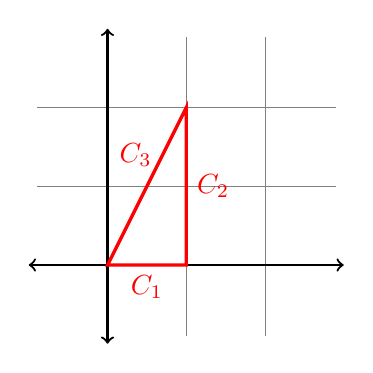
\begin{tikzpicture}
    \draw[step=1cm,gray,very thin] (-0.9,-0.9) grid (2.9,2.9);
    \draw[thick,<->] (-1,0) -- (3,0);
    \draw[thick,<->] (0,-1) -- (0,3);
    \draw[red,very thick] (0,0) -- (1,0) node[below,pos=0.5] {\( C_1 \)}
      -- (1,2) node[right,pos=0.5] {\( C_2 \)}
      -- cycle node[left,pos=0.3] {\( C_3 \)};
  \end{tikzpicture}
\end{center}
\begin{align*}
  \oint_{C}xy\diff{x}+x^2y^3\diff{y} &=
    \int_{C_1}xy\diff{x}+x^2y^3\diff{y}+
    \int_{C_2}xy\diff{x}+x^2y^3\diff{y}+
    \int_{C_3}xy\diff{x}+x^2y^3\diff{y} \\
  &= \int_{C_1}0\diff{x}+0+
    \int_{C_2}0+y^3\diff{y}+
    \int_{C_3}\frac{y}{2}y\frac{\diff{y}}{2}+(\frac{y}{2})^2y^3\diff{y} \\
  &= 0+\int_{0}^{2}y^3\diff{y}+
    \int_{2}^{0}\frac{y^2}{4}\diff{y}+\frac{y^5}{4}\diff{y} \\
  &= 0+\bigg[\frac{y^4}{4}\bigg]_{0}^{2}+
    \bigg[\frac{y^3}{12}+\frac{y^6}{24}\bigg]_{2}^{0} \\
  &= 4-\frac{2}{3}-\frac{8}{3} \\
  &= \frac{2}{3} \\
  \oint_{C}xy\diff{x}+x^2y^3\diff{y} &=
    \iint_{D}\left(\pdiff{Q}{x}-\pdiff{P}{y}\right)\diff{A} \\
  &= \int_{0}^{1}\int_{0}^{2x}-x+2xy^3\diff{y}\diff{x} \\
  &= \int_{0}^{1}\bigg[-xy+\frac{xy^4}{2}\bigg]_{0}^{2x}\diff{x} \\
  &= \int_{0}^{1}-2x^2+8x^5\diff{x} \\
  &= \bigg[-\frac{2x^3}{3}+\frac{8x^6}{6}\bigg]_{0}^{1} \\
  &= -\frac{2}{3}+\frac{8}{6} \\
  &= \frac{2}{3}
\end{align*}

\subsubsection*{Exercise 7}
Use Green's Theorem to evaluate the line integral along the given positively
oriented curve.
\[ \int_{C}(y+\e^{\sqrt{x}})\diff{x}+(2x+\cos(y^2))\diff{y} \]
\( C \) is the boundary of the region enclosed by the parabolas \( y = x^2 \)
and \( x = y^2 \).
\begin{align*}
  \oint_{C}P\diff{x}+Q\diff{y} &=
    \iint_{D}\left(\pdiff{Q}{x}+\pdiff{P}{y}\right)\diff{A} \\
  &= \int_{0}^{1}\int_{x^2}^{\sqrt{x}}(2-1)\diff{y}\diff{x} \\
  &= \int_{0}^{1}\bigg[y\bigg]_{x^2}^{\sqrt{x}}\diff{x} \\
  &= \int_{0}^{1}\sqrt{x}-x^2\diff{x} \\
  &= \bigg[\frac{2x^{\frac{3}{2}}}{3}-\frac{x^3}{3}\bigg]_{0}^{1} \\
  &= \frac{2}{3}-\frac{1}{3} = \frac{1}{3}
\end{align*}

\subsubsection*{Exercise 13}
Use Green's Theorem to evaluate \( \int_{C}F\cdot\diff{r} \).
\[ F(x,y) = \langle y-\cos(y),x\sin(y)\rangle \]
\( C \) is the circle \( (x-3)^2+(y+4)^2 = 4 \) oriented clockwise.
\begin{align*}
  \oint_{C}P\diff{x}+Q\diff{y} &=
    \iint_{D}\left(\pdiff{Q}{x}+\pdiff{P}{y}\right)\diff{A} \\
  &= \iint_{D}\sin(y)+1-\sin(y)\diff{x}\diff{y} \\
  &= \int_{0}^{2}\int_{0}^{2\pi}r\diff{\theta}\diff{r} \\
  &= \int_{0}^{2}\bigg[r\theta\bigg]_{0}^{2\pi}\diff{r} \\
  &= \int_{0}^{2}2\pi r\diff{r} \\
  &= \bigg[\pi r^2\bigg]_{0}^{2} \\
  &= 4\pi
\end{align*}

\subsubsection*{Exercise 17}
Use Green's Theorem to find the work done by the force
\( F(x,y) = x(x+y)\i+xy^2\j \) in moving a particle from the origin along the
x-axis to (1,0), then along the line segment to (0,1), and then back to the
origin along the y-axis.
\begin{center}
  \begin{tikzpicture}[scale=2]
    \draw[step=1cm,gray,very thin] (-0.9,-0.9) grid (1.9,1.9);
    \draw[thick,<->] (-1,0) -- (2,0);
    \draw[thick,<->] (0,-1) -- (0,2);
    \draw[red,very thick] (0,0) -- (1,0) -- (0,1) -- cycle;
  \end{tikzpicture}
\end{center}
\begin{align*}
  \oint_{C}P\diff{x}+Q\diff{y} &=
    \iint_{D}\left(\pdiff{Q}{x}+\pdiff{P}{y}\right)\diff{A} \\
  &= \iint_{D}y^2-x\diff{A} \\
  &= \int_{0}^{1}\int_{0}^{1-x}y^2-x\diff{y}\diff{x} \\
  &= \int_{0}^{1}\bigg[\frac{y^3}{3}-xy\bigg]_{0}^{1-x}\diff{x} \\
  &= \int_{0}^{1}\frac{(1-x)^3}{3}-x(1-x)\diff{x} \\
  &= \int_{0}^{1}\frac{1-3x+3x^2-x^3}{3}-x+x^2\diff{x} \\
  &= \int_{0}^{1}\frac{1}{3}-x+x^2-\frac{x^3}{3}-x+x^2\diff{x} \\
  &= \int_{0}^{1}-\frac{x^3}{3}+2x^2-2x+\frac{1}{3}\diff{x} \\
  &= \bigg[-\frac{x^4}{12}+\frac{2x^3}{3}-x^2+\frac{x}{3}\bigg]_{0}^{1} \\
  &= -\frac{1}{12}+\frac{2}{3}-1+\frac{1}{3} \\
  &= -\frac{1}{12}
\end{align*}

\begin{center}
  If you have any questions, comments, or concerns, please contact me at
  alvin@omgimanerd.tech
\end{center}

\end{document}
